\documentclass{article}
\author{Jake Lane}
\title{Optimising Higgs Decay events to Background events in the di-photon channel}
\usepackage{amsmath, graphicx, listings	}
\graphicspath{{../figures/}}

\begin{document}
\maketitle
\begin{abstract}
A Higgs decay in to 2 photons ($H \rightarrow \gamma \gamma$) is optimised against a background of 2 photons simulated by python as gluon decay into 2 photons ($g \rightarrow \gamma \gamma$.) The signal was optimised via filtering the events based on their kinematic variables. The weighted results presented no evidence of the existence of a particle compared to a background photon, weighted results do result in a peak around the $m_H = 125$ GeV but are obscured by a larger peak where the background most likely survived the filtering. 
\end{abstract}
\section{Introduction}
The aim of this project was to optimise a signal produced a program called Pythia of a decay of a Higgs boson ($H$) to 2 photons ($\gamma$.) This report will summarise the results of the project, justify the theoretical and experimental reasoning for the methods used to obtain these results and comment on the results obtained compared to current literature. \cite{HiggsDetection}
To begin a theoretical background is given first to illustrate the relevant theory being examined. The way in which the data is processed is then discussed in context of the physical processes being examined. The results are then presented in graph form, using both 3D scatter plots (for the optimisation plot) and 2D histogram plots (for the invariant mass plot). Comments on the results as well as comparison to current literature will then follow; the project's experimental (and theoretical) faults will be examined and improvements on these faults will be offered. The conclusion will summarise the results and comments in context of the literature as well as summarising the faults and possible improvements that could be made.  
\section{Theory}
\subsection{Higgs Mechanism}
The Higgs mechanism, as proposed by Higgs, allowed for particles to keep their masses and keep the symmetry of the Standard Model Electroweak interaction via symmetry breaking with a scalar field (called the 'Higgs' Field) that permeates all of space.\cite[p.~1159]{peterHiggs66} The details of the Higgs interaction (and electroweak theory) are not needed to optimise the signal, however the decay of the Higgs boson (that arises out of the introduction of the Higgs mechanism) affected by how the Higgs field 'couples' to other particles (in particular the photon and top quark.)
\subsection{Higgs Decay}
The Higgs boson has many possible decay modes, as it is estimated to have a relatively large mass in the window of $113 < m_H < 132 GeV/c^2$ at the 95\% confidence limit. The most common decay for the Higgs boson is into a bottom, anti-bottom quark pair:
\begin{equation}
H \rightarrow b \bar{b}
\end{equation}
The decay we are interested in is the Higgs boson to 2 photons (or the 'di-photon channel'):
\begin{equation}
H \rightarrow \gamma \gamma
\end{equation}
\cite{HiggsdecayEMback}
%refer to Higgs decay theory
This decay has a very low chance of occurring, with a branching fraction of order $10^{-3}$ times per decay. \cite[p.~5]{HiggsCross3} The decay of the Higgs to the 2 photons is unlikely due to the nature of the decay, since the photon (having no mass) does not couple to the Higgs field, the only way to produce 2 photons from a Higgs is for the Higgs to decay into 2 particles (usually 2 top quarks \footnote{Other particle pairs can and are produced but at such low branching fractions that they are negligible}) which then annihilate to produce 2 photons. 
\begin{figure}
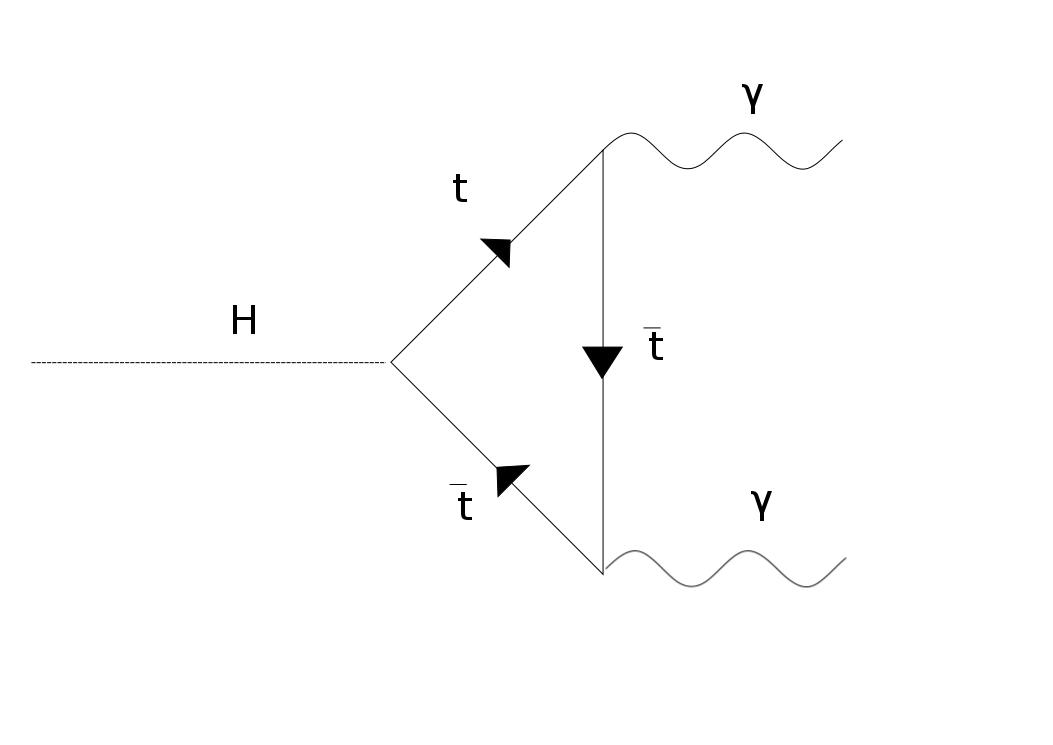
\includegraphics[scale=0.25]{Hyy}
\caption{Feynman diagram for $H \rightarrow \gamma \gamma$ decay channel via a top quark loop}
\end{figure}
This decay is far less common than the decay to a bottom-anti bottom quark pair with a branching fraction of order $10^{0}$ \cite[p.~5]{HiggsCross3}. It is reasonable to wonder why the botton-antibottom quark decay channel was not explored instead of the di-photon channel, it is for practical purposes that the di-photon channel is preferred. As quarks cannot be isolated, the decayed bottom-anti-bottom quark pair would manifest in a 'jet' of hadrons which would require a far more complex analysis of each event for possible candidate Higgs decays, contrast to a di-photon decay where 2 photons can be isolated and do not have associated jets, it is relatively simple to identify 2 candidate photons for Higgs decay than it is to do so for a bottom-anti bottom quark decay. 
\subsection{Significance}
In order to test the effectiveness of the optimisation of the signal to background a quantitative measurement was needed, the statistical significance, $\Sigma$ is given by the number of events $S$ compared a background of number of events, $B$.
\begin{equation}
\Sigma = \frac{S}{\sqrt{S + B}} 
\end{equation}
Note that the significance is inversely proportional to the inverse square root of the total number of events, $N = S + B$, meaning that scaling to larger number of events would yield a lower significance at a relatively fast pace. Also note that reducing the number of background events, $B$ to it's lowest ($B = 0$) would give a maximum value of $\Sigma = 1$, assuming that the signal is purely Higgs boson decays. On inspection of the signal data ('Higgs.txt') it is clear from the non-zero number of single photon events that the signal was not purely Higgs decays and needed filtering as well as the background. 
\subsection{Kinematics}
As the Higgs is produced in our simulation at a LHC-like collider experiment, there are kinematic variables introduced to parameterise the Energy and momentum (4 - momenta) of the produced photons. These are given by the transverse momentum $p_T$, the azimuthal angle $\phi$ and the pseudo-rapidity $\eta$ (in this case the pseudo-rapidity is the rapidity see appendix) related to the energy and 3 cartesian components of the momentum vector of the photon by
\begin{align}
E &= p_T \cosh {\eta} \\
p_x &= p_T \cos{\phi} \\
p_y &= p_T \sin{\phi} \\
p_z &= p_T \sinh{\eta}
\end{align}
The reasoning behind using the transverse momentum is that it is Lorentz invariant as the particles are only moving relativistically along the beam line, perpendicular to the transverse momentum. The differences in $\phi$ and $\eta$ are also Lorentz invariant and allow for a measure of the angular distance between photons. The difference in azimuthal angle, the angle in the plane perpendicular to the beam line, would test to see if the Higgs decays into 2 back to back photons (preserving transverse momentum) and the pseudo-rapidity difference allows for a measure of angle along the beam axis that is Lorentz invariant.
\subsection{Higgs invariant mass}
The way in which the Higgs signal will manifest is via an 'invariant mass plot' where the frequency of the an event of invariant mass $m$ against the invariant mass. 
The Higgs to 2 photon decay event is relativistic and requires the conservation of the magnitude of the 4-momentum, $p_H^\mu$, where $\mu = t, x, y, z$ for a 4-vector. Which leads to the relation
\begin{equation}
m_H^2 = 2 E_{\gamma 1} E_{\gamma 2} (1 + \cos(\phi_1 - \phi_2)) 
\end{equation}.
This equation is used to obtain the expected parameters of the di-photon channel, therefore it is possible to distinguish background produced photons and Higgs produced photons. 
From (8), assuming that the transverse momenta and the energy are of the same order of magnitude and that $(1 + cos(\phi_1 - \phi_2)) \approx 1$ then it is expected that photons from a Higgs decay will have $p_T \approx m_H$.
\subsection{Weighting}
The Higgs signal is artificially large compared to the background on it's own and must be weighted to correspond to a physically realistic proportion of decays in a background this is done using the weighting, $w_H$,  for a Higgs decay
\begin{equation}
w_H = \frac{\sigma_{H}}{\sigma_{B}} B(H \rightarrow \gamma \gamma)
\end{equation}
Where $\sigma_H, \sigma_B$ are the cross sections (which are roughly related to probability) of Higgs production and background photon production respectively whilst $B(H \rightarrow \gamma \gamma)$ is the branching ratio for Higgs decay to 2 photons. 
\subsection{Expectation}
Since the current search for Higgs boson yielded a result of $5\sigma$ at mass $m_H = 126^{+ U}_{-L}$GeV at ATLAS combined with the exclusion by the LEP and Tevatron in the range $113 < m_H < 132$ GeV respectively to the 95\% confidence limit; we expect a peak in a invariant mass Histogram within the range described and near the $125$ GeV from ATLAS.
%refer to kinematic textbook
\section{Coding}
%Aka method
\subsection{Parsing}
In order to begin to manipulate 4 momenta data, we needed that data to be in a usable format; this was done via a python script called 'parse.py' (as seen in appendix A.1) The parsing program would proceed through both the 'Higgs.txt' file containing the photon event data for a Higgs signal and the 'background.txt' file which had the background photon events that the Higgs signal was optimised to. The script would take the following information from the text file for each 'event.':
\begin{enumerate}
\item The number of photons $n$ for each event.
\item Each component of the 4-momentum, $p_x, p_y, p_z$ for the $x, y, z$ directions for each photon
\item The energy, $E$ of each photon in the event
\end{enumerate}
The format of this information was a python 'class' which allowed each event to treated as an object to be manipulated by further programs.
\subsection{Filtering}
The filtering functions work on the following algorithm
%Will be a flowchart
\begin{enumerate}
\item The photon has property $x$
\item $x$ satisfies an inequality $I(x, X)$
\item Event with photon with $x$ is kept.
\item Otherwise photon is discarded (not kept).
\item Events with fewer than 2 photons are discarded.
\end{enumerate}
In the case where more than 2 photons survive the filtering process, another means is used to select 2 of the best photons that meet these criteria depending on the physical quantity being filtered.
\subsection{Filters}
\subsubsection{Number}
The number of photons in each event is calculated by iterating through the list of events and finding the number of photons in each event. The event is rejected if there are fewer photons than a threshold number $n$. In our case $n=2$ since the Higgs cannot possibly decay into fewer than 2 photons, this means that the events are filtered by number both before filtering and after filtering to avoid non-Higgs candidates being present in the final array of events. 
\subsubsection{Transverse Momentum}
The transverse momentum filter iterates through all of the events as stored by 'parse.py' (appendix A.1) in a list and keeps every event but removes all photons from that event that have a transverse momentum $p_T < P_T$ where $P_T$ is obtained via optimising the filter with respect to the statistical significance of the Higgs signal $\Sigma$. 
In the case of more than 2 eligible photons, the photons with the highest $p_T$ were chosen since these are more likely to be the result of a Higgs decay. 
\subsubsection{Energy}
As with the transverse momenta filter, the energy filter will also remove every photon with Energy $E< E_{th}$ , where $E_{th}$ is some threshold energy also obtained by optimising the energy filter. 
\subsubsection{Azimuthal angle}
The azimuthal angle filter considers each event and 2 photons in the event with 4-momenta $p_i, p_j$ and proceeds to find the angle $\phi_{ij}$ between them. To avoid repeating the same operation only events with $i+j<1$ are chosen so that the angle is taken between different photons a single time between them.
\subsubsection{Pseudo-Rapidity}
The pseudo rapidity was filtered in the same manner as the azimuthal angle, where 2 photon 4-momenta are considered and the pseudo rapidity is taken between them.
\subsection{Optimisation}
To optimise each of the filters, the Higgs events and background events are filtered several times and have the statistical significance, $\Sigma$ recorded at each value of the threshold value of each filter. This means that the statistical significance $\Sigma$ is a function of minimum transverse momenta $p_{T1}, p_{T2}$, minimum energy, $E_1, E_2$, minimum azimuthal angle $\phi$ and minimum pseudo rapidity $\eta$.
\begin{equation}
\Sigma = \Sigma(p_{T1}, p_{T2}, E_1, E_2, \phi, \eta)
\end{equation}
To find the largest value of $\Sigma$, we find the largest value by changing each of the variables that $\Sigma$ depends on. We do this by plotting $\Sigma$ against a range of values of each variable and finding the maximum value of $\Sigma$ from each one. Then the combination of all of these parameters are used to filter the events and produce an invariant mass plot.
\subsection{Plotting}
The invariant mass plot is used via the 'pyplot' library, creating a histogram of the invariant masses, calculated from the events using the summation of 4-momenta and taking the square as
\begin{equation}
m_{\gamma \gamma}^2 = (E_1 + E_2)^2 - ({\bf p}_1  + {\bf p}_2)^2
\end{equation}
\section{Results}
\subsection{Optimisation}
\subsubsection{Transverse Momenta}
\begin{figure}
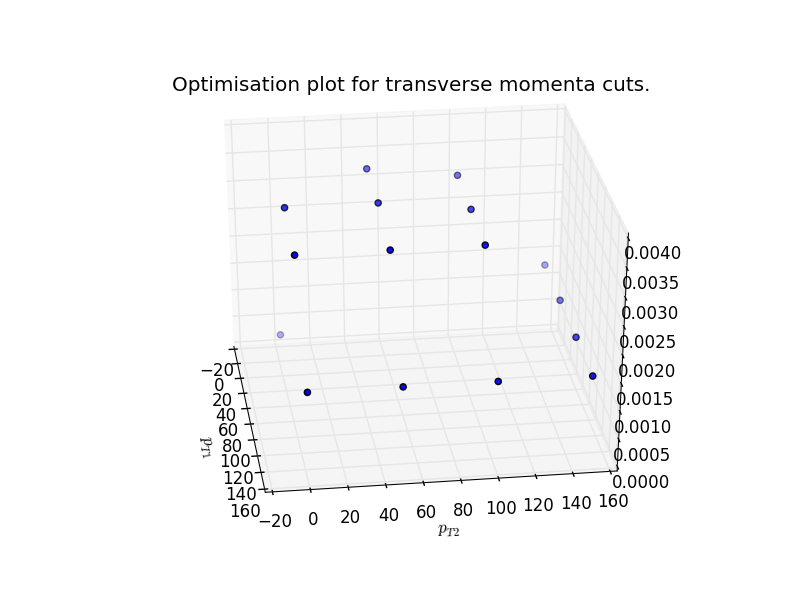
\includegraphics[scale=0.5]{transverse6}
\caption{Statistical signifiance dependence on transverse momenta}
\end{figure}

As shown in figure 2, the significance plateaus starting at $p_{T1} = p_{T2} = 90$ GeV. It is noticeable that the significance has decreased before the $p = 120$GeV value, as expected from the kinematics of the Higgs decay, this would suggest that there is some other factor we have missed from the filtering. It may be the case that the competing decay (2 gluon to 2 photons) dominates from the background at such a high amount that optimising the Higgs signal is not possible since there are so few candidates to be Higgs to 2 photons yet still have many background eligible candidates. A solution to this could be a matter of building up the background to compare to the Higgs signal (starting from only the Higgs signal) instead of simply mixing the 2 sources together, whilst this does not reflect the reality of a collider experiment, it would give us the chance to optimise the signal and find out where the background drowns out the signal.
\subsubsection{Energy}
\begin{figure}
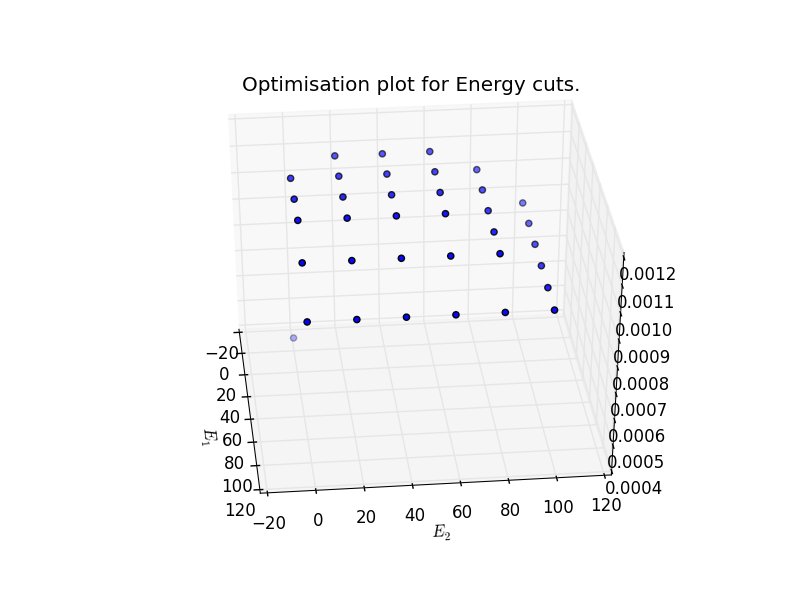
\includegraphics[scale=0.5]{energy6}
\caption{Energy dependence of significance}
\end{figure}
In figure 3, there is also a plateau for energy with respect to significance similar to that of the transverse momentum, this is to be largely expected since the expectation for the pseudo-rapidity of the photons was expected to be near $0$ since the photons would decay back to back. This means that the energy would be similar to transverse momentum. 
\subsubsection{Azimuthal angle and Pseudo-rapidity}
\begin{figure}
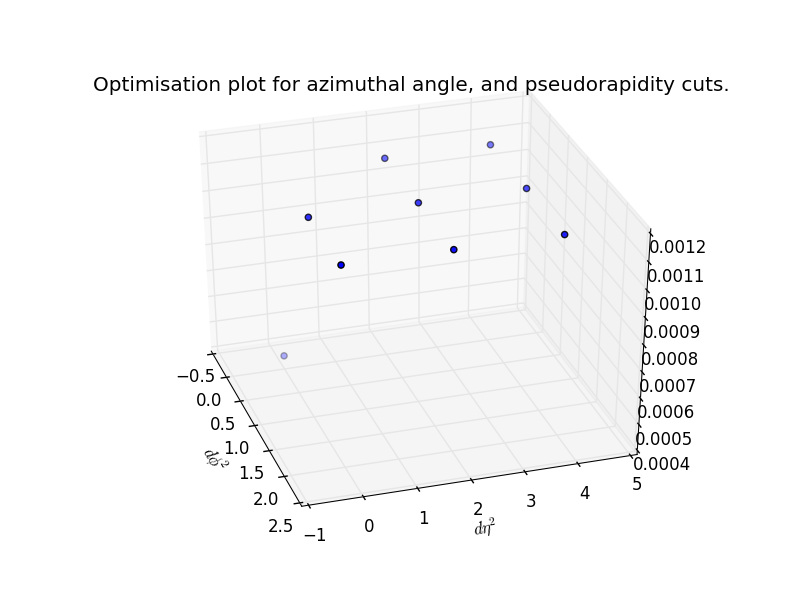
\includegraphics[scale=0.5]{etaphi1}
\caption{Azimuthal angle and pseudo-rapidity dependence on $\Sigma$}
\end{figure}
The azimuthal angle dependance is more surprising than the pseudo-rapidity result since we expected a peak near a 'back to back' angle of $\Delta \phi = \frac{\pi}{2}$ since we obtain only a dependance on eta, again reaching a plateau. This also suggests that the filtering did not fully eliminate background to Higgs decays. 
%Comment about the inv mass plot before + after optimisation
\subsection{Invariant mass}
The resulting invariant mass plots from no filtering at all (figure 5) compared to the optimised filtering as discussed in section 4.1 yields the important distinction that there are far fewer events as a result of filtering, which suggests that the filtering has been to some extent selective in choosing photons, furthermore a peak of sorts is observed near the $m_{\gamma \gamma}=125$GeV region, however this is obscured by a larger peak near the $m_{\gamma \gamma} = 200$ GeV, which would suggest that the background is still contributing high energy photons to the invariant mass plot (and inspecting the lack of a 'width' for this peak.) This is likely solved by iterating over all of the invariant masses of the background and excluding the larger invariant masses (specifically where the Higgs boson mass is excluded at the 95\% CL.) 
\begin{figure}
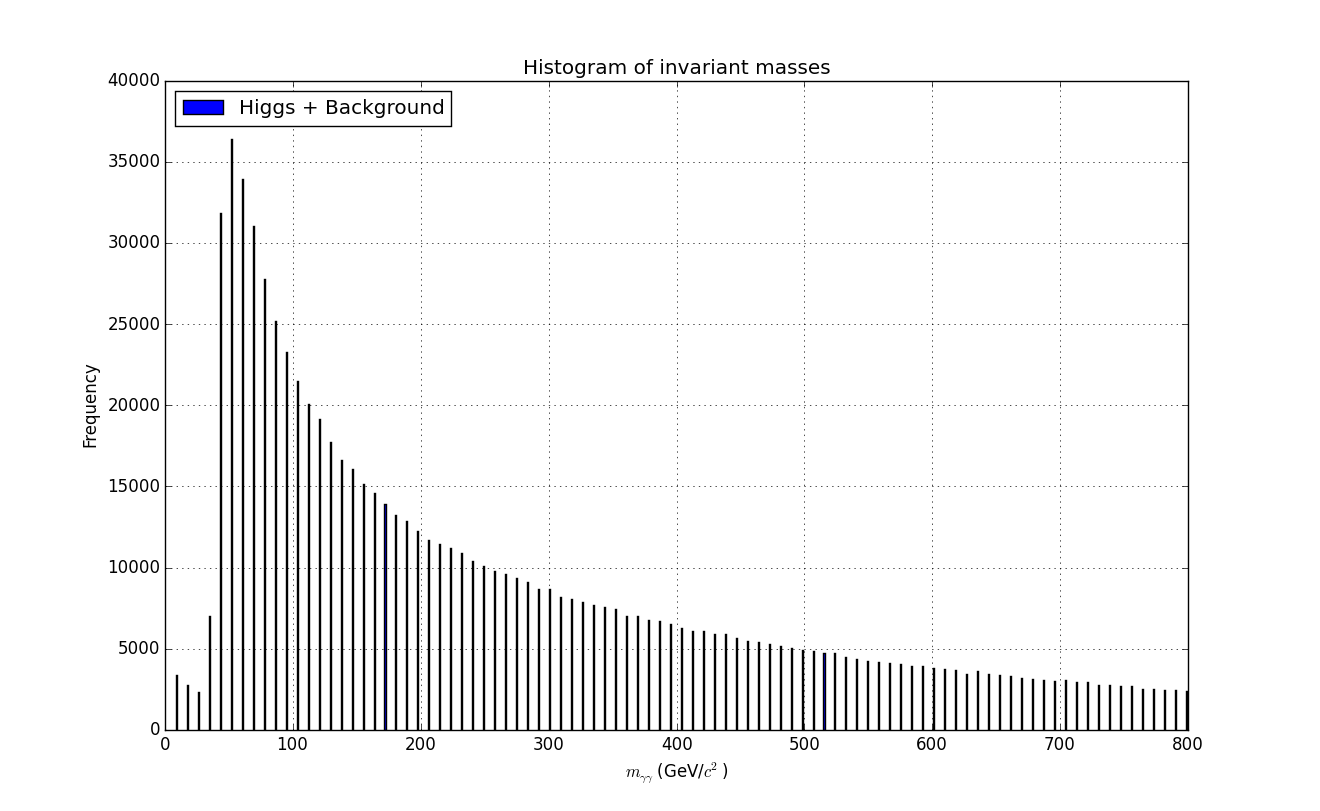
\includegraphics[scale = 0.3]{First_unfiltered_invmass}
\caption{Unfiltered invariant mass plot}
\end{figure}
\begin{figure}
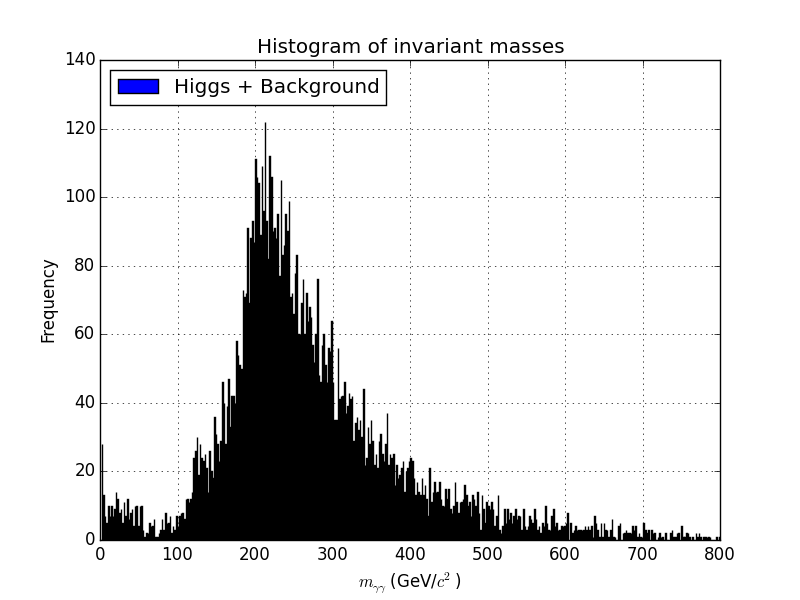
\includegraphics[scale = 0.5]{First_filtered_invmass}
\caption{Filtered invariant mass plot}
\end{figure}

\section{Conclusion}
The overall result of this project was that a signal was optimised in comparison to a given background. The consideration of the physical parameters that govern the decay of the Higgs allowed for this optimisation to take place. The following analysis of this new optimised signal was still a noisy data set, which would suggest that the filtering is incomplete with respect to the known limits of the Higgs mass. It would be an improvement to the filtering process if such a mass window was implemented to the final filtering mechanism. Whilst there was a peak produced where the Higgs boson would likely show a peak, it is not reasonable to say that this peak is at all significant. The result from this project as such should be seen as a negative result for observing a Higgs under the current filtering process. 
\bibliographystyle{plain}
\bibliography{reference}
\appendix
\section{Code}
\subsection{Parse.py}
%Put code in here
\begin{lstlisting}
#!/usr/bin/env python3

import sys, argparse, pickle
import matplotlib.pyplot as plt
from multiprocessing import Pool

from fourmomentum import FourMomentum
from event import Event


#Number filter (more than n events)
def number_threshold(events, n):
    """ Filters events so that only events with more than
        n momenta are returned. """
    return list(filter(lambda x: len(x) > n, events))

#Transverse momentum filter
def transverse_threshold(events, p_T):
    new_events = []
    for event in events:
        if len(list(filter(lambda x: x.transverse() > p_T, event.momenta))) > 0:
            new_events.append(event)
    return new_events

#Keeps the 20GeV transverse momentum
def transverse_threshold_2(events, p_T):
    events2 = []
    for event in events:
        for momenta in event.momenta:
            # If there are any transverse momenta > p_T, that event is valid
            if momenta.transverse() > p_T:
                events2.append(event)
                break
    return events2

#Energy filter
def energy_threshold(events, E):
    new_events = []
    for event in events:
        if len(list(filter(lambda x: x.energy > E, event.momenta))) > 0:
            new_events.append(event)
    return new_events

def energy_threshold_2(events, E):
    events2 = []
    for event in events:
        for momenta in event.momenta:
            if momenta.energy > E:
                events2.append(event)
                break
    return events2

def deta_threshold(events, eta):
    res = list(filter(lambda x: x.eta_diff_max() > eta**2, events))
    return res

def dazi_threshold(events, azi):
    return list(filter(lambda x: x.azi_diff_max() > azi**2, events))

def invmass_threshold(events, m):
    return list(filter(lambda x: x.invariant_mass()>m, events))

def invmass_limit(events, m):
    return list(filter(lambda x: x.invariant_mass() < m, events))

#combined filter
def combined_filter(events, num=1, momentum_lower=4, momentum_higher=50, energy_lower=20, energy_higher = 20,
                    deta = 0, dazi = 0, invm1 = 100, invm2 = 1000):
    #Filtering events
    #only show events with at least 2 momenta
    res = number_threshold(events, num)
    print("Number filtered")
    #Exclude in lower invariant mass range
    res = invmass_threshold(res, invm1)
    print("Lower Inv mass filtered")

    res = transverse_threshold(res, momentum_lower)
    res = transverse_threshold_2(res, momentum_higher)
    print("Momenta filtered")

    res = energy_threshold(res, energy_lower)
    res = energy_threshold_2(res, energy_higher)
    print("Energy filtered")

    # Pick the two highest transverse momenta from the event
    for event in res:
        event.filter_highest_pt(2)

    print('Chose 2 highest p_T photons')
    #res = deta_threshold(res, deta)
    print("Pseudorapidity filtered")
    #res = dazi_threshold(res, dazi)
    print("Azimuthal filtered")

    for event in res:
        if len(event) > 2:
            raise ValueError

    #Exclude higher invariant mass range
    #res = invmass_limit(res, invm2)
    print('Upper invariant mass')
    print("Finished filtering")
    return res

def get_invariant_masses(events):
    invariant_masses = []
    for i, event in enumerate(events):
        invariant_masses.append(event.invariant_mass())
    return invariant_masses

def parse_file(path, count=False, momenta_in_event=False):
    """ Parse the event file with name path returning Event objects.

        Keyword arguments:
        path  -- The filepath of the event file
        count -- Whether to print the current num. processed events
        momenta_in_event -- Whether to use file containing num. four
                            momenta in each event.

        The four momenta count file should have the filename path + '_count'
        and each line should contain the number of four momenta in each
        event of the events file (as specified in the path argument) in
        order of event appearance (the first number in the count file
        has the number of four momenta in the first event of the events file)."""

    events = []
    with open(path) as data_file:
        raw = data_file.read().split('\n')

        if momenta_in_event:
            count_file = open(path + '_count')
            counts = count_file.read().split('\n')
            # Current event number in file
            current_event_number = 0

        four_momenta_count = 0
        counter = 0
        p = Pool(100)
        for i, line in enumerate(raw):
            # If the line starts with 'Event', begin to process it
            if line.startswith('Event'):
                # If number of momenta given, use that, else just use 20
                if momenta_in_event:
                    four_momenta_count = int(counts[current_event_number])
                    current_event_number += 1
                else:
                    four_momenta_count = 20

                new_event = Event.from_text(raw[i+1:i+four_momenta_count])
                p.apply_async(events.append(new_event))
                #events.append(Event.from_text(raw[i:i+10]))

                if count:
                    counter += 1
                    if counter % 1000 == 0:
                        print(counter)

    return events



def main():
    parser = argparse.ArgumentParser(description='Generate histogram from Higgs event data')
    parser.add_argument('--higgs', nargs=1, default='higgs.txt', metavar='path_to_higgs',
                        dest='higgs_path', help='Relative path to higgs data')
    parser.add_argument('--background', nargs=1, default='background.txt', metavar='path_to_background',
                        dest='background_path', help='Relative path to background data')
    parser.add_argument('--print_higgs', action='store_true',
                        help='Whether to print the calculated invariant masses of the Higgs signal to stdout.')
    parser.add_argument('--print_bkg', action = 'store_true',
                        help='Whether to print the calculated invariant masses of the background to stdout.')
    parser.add_argument('--parsed_higgs', action='store_true',
                        help='Print parsing information of Higgs signal to stdout.')
    parser.add_argument('--parsed_bkg', action='store_true',
                        help='Print parsing information of background to stdout.')
    parser.add_argument('--count', action='store_true',
                        help='Whether to print current line of parsing.')
    parser.add_argument('--momenta_count_in_event', action='store_false',
        help="""Don't use files which hold the number of events in the event,
                with the name of the datafile + '_count'.""")
    parser.add_argument('--onlyhiggs', action='store_true',
        help="""Only use the Higgs file (don't parse the background)""")
    parser.add_argument('--opt', action = 'store_true', help = 'uses optimised values')

    args = parser.parse_args()
    default_param = [90, 90, 50, 50, 0, 0, 100000]
    #default_param = [0, 0, 0, 0, 0, 0, 0]
    p_T1, p_T2, E_1, E_2, dphi, deta, m = default_param

    if args.opt:
        opt_param = open('optimised.txt', 'r').read().split(',')
        opt_param = list(map(lambda x: float(x), opt_param))
        p_T1, p_T2, E_1, E_2, dphi, deta, m, m2 = opt_param

    # Higgs signal
    higgs_events = parse_file(args.higgs_path, count=args.count,
            momenta_in_event=args.momenta_count_in_event)
    print("Parsed higgs")
    higgs_events = combined_filter(higgs_events, num = 1, momentum_lower = p_T1, momentum_higher = p_T2, energy_lower = E_1, energy_higher = E_2,
                                   deta = deta, dazi = dphi)
    print("Filtered higgs")
    invariant_masses_higgs = get_invariant_masses(higgs_events)
    print("Got invariant masses higgs")

    # Background signal
    if not args.onlyhiggs:
        bkg_events = parse_file(args.background_path, count=args.count,
                momenta_in_event=args.momenta_count_in_event)
        print("Parsed background")
        bkg_events = combined_filter(bkg_events, num = 1, momentum_lower = p_T1, momentum_higher = p_T2, energy_lower = E_1, energy_higher = E_2,
                                       deta = deta, dazi = dphi)
        print("Filtered background")
        invariant_masses_bkg = get_invariant_masses(bkg_events)
        invariant_masses_combined = invariant_masses_higgs + invariant_masses_bkg
        print("Got invariant masses background")
    else:
        invariant_masses_combined = invariant_masses_higgs

    if args.print_higgs:
        for mass in invariant_masses_higgs:
            print(mass)

    if args.print_bkg:
        for mass in invariant_masses_bkg:
            print(mass)

    if args.parsed_higgs:
        for event in higgs_events:
            print(event.momenta)
            print('Event', event.id)
            for momenta in event.momenta:
                print('Energy:', momenta.energy)
                print('p_T:', momenta.transverse())

            print('Invariant mass:', invariant_mass)

    if args.parsed_bkg:
        for event in bkg_events:
            print(event.momenta)
            print('Event', event.id)
            for momenta in event.momenta:
                print('Energy:', momenta.energy)
                print('p_T:', momenta.transverse())

            print('Invariant mass:', invariant_mass)

    print("Writing invariant masses to file")
    if args.onlyhiggs:
        #out_higgs = open('outputIM_Higgs.txt', 'r+')
        #out_higgs.truncate()
        #out_higgs.close()
        out_higgs = open('outputIM_Higgs.txt', 'w')
        out_higgs.write(str(invariant_masses_higgs))
    else:
        #out_bkg = open('outputIM_bkg.txt', 'r+')
        #out_bkg.truncate()
        #out_bkg.close()
        #out_cmb = open('outputIM_cmb.txt', 'r+')
        #out_cmb.truncate()
        #out_cmb.close()
        with open('outputIM_Higgs.txt', 'wb') as f:
            pickle.dump(invariant_masses_higgs, f)
        with open('outputIM_bkg.txt', 'wb') as f:
            pickle.dump(invariant_masses_bkg, f)
        with open('outputIM_cmb.txt', 'wb') as f:
            pickle.dump(invariant_masses_combined, f)

if __name__ == '__main__':
    main()



\end{lstlisting}
\subsection{Significance.py}
\begin{lstlisting}
#!/usr/bin/env python3

from math import sqrt
from math import radians
import parse
import matplotlib.pyplot as plt
from mpl_toolkits.mplot3d import Axes3D
import argparse

def get_largest(z, x, y):
    if len(z) == 0:
        return [0, 0, 0]

    z_max = max(z)
    index = z.index(z_max)
    x_max = x[index]
    y_max = y[index]
    return [x_max, y_max, z_max]

def statistical_significance(signal, background):
    """ Calculate statistical significance given num. signal events
        and num. background events. """
    cs_H = 17.35
    br_yy = 2.28e-3
    cs_bkg = 140.
    w = cs_H * br_yy/cs_bkg
    if signal == 0:
        return 0
    else:
        return signal * w / sqrt(signal * w + background)

def main():
    parser = argparse.ArgumentParser(description="""Generate 2D histogram of
                        statistical significance of various filters.""")
    parser.add_argument('--back', action='store_false',
                        help="Don't use the background.")
    parser.add_argument('--transverse', action='store_true', help='transverse cuts')
    parser.add_argument('--energy', action = 'store_true', help = 'energy cuts')
    parser.add_argument('--etaphi', action = 'store_true', help = 'cuts both azimuthal and psudeorapidity difference squared')
##    parser.add_argument('range2D', metavar = 'range2D', type = int, nargs = '+',
##                       help = 'choose x-axis for plot, xmin xmax step ymin ymax step')
    parser.add_argument('--out_opt', action = 'store_false', help = 'outputs invarant masses of optimised results')
    parser.add_argument('--plot', action = 'store_true', help = 'plots the optimisation')
    parser.add_argument('--nopreset', action = 'store_false', help = "don't use optimisation data")
    parser.add_argument('--choose_range', action = 'store_false', help = 'takes the old optimised value (from a previous run) and looks 2 parameters (at a chosen resolution)')
    args = parser.parse_args()
    xlabel = ''
    ylabel = ''
    title = ''

    xrange = [0, 100, 20]
    yrange = [0, 100, 20]



##    if not args.choose_range:
##        xrange = args.range2D[0:3]
##        if len(xrange)<3:
##            xrange = [0, 100, 20]
##        yrange = args.range2D[3:len(args.range2D)]
##        if len(yrange) < 3:
##            yrange = [0, 100, 20]
    # Get all the events
    m = 0
    higgs_events = parse.parse_file('higgs.txt', momenta_in_event=True)

    res = 0.05
    filtered_higgs = {}
    default_param = [90, 90, 50, 50, 0, 0, 113, 132]
    opt_p_T1, opt_p_T2, opt_E_1, opt_E_2, opt_dphi, opt_deta, m1, m2 = default_param

    ranges = [
            range(0, 200, 50),
            range(0, 200, 50),
            range(1, 11, 2),
            range(1, 11, 2),
            range(0, 6, 2),
            range(0, 3, 1),
         ]

    # Preset optimised values
    if args.nopreset:
        param = open('optimised.txt', 'r').read().split(',')
        param = list(map(lambda x: float(x), param))
        opt_p_T1, opt_p_T2, opt_E_1, opt_E_2, opt_dphi, opt_deta, m1, m2 = param

        # When you use an automatic range, use these parameters
        # Each range corresponds to the default ranges for each filter
        # in order: transverse momenta 1 & 2, energies 1 & 2, azimuthal, pseudorapidity
        ranges = [
                    range(60, 120, 30),
                    range(60, 120, 30),
                    range(0, 101, 20),
                    range(0, 101, 20),
                    range(0, 6, 2),
                    range(0, 3, 1),
                 ]

        if args.choose_range:
            lim = input('Outer limits for optimisation: ')
            lim = float(lim)

            a = [-lim, 0, lim]
            ranges = []
            for p in param:
                ranges.append(list(map(lambda x: x + p, a)))

            print(ranges)

    if args.back:
        bkg_events = parse.parse_file('background.txt', momenta_in_event=True)
        filtered_bkg = {}

    if args.transverse:
    # Apply a series of different filters in turn
##        lower_momentum = range(xrange[0], xrange[1], xrange[2])
##        higher_momentum = range(yrange[0], yrange[1], yrange[2])
        lower_momentum = ranges[0]
        higher_momentum = ranges[1]
        xlabel = '$p_{T1}$'
        ylabel = '$p_{T2}$'
        title = 'transverse momenta'
        for lower in lower_momentum:
            for higher in higher_momentum:
                filtered_higgs[(lower, higher)] = parse.combined_filter(higgs_events,
                                                                        num=1, momentum_lower=lower,
                                                                        momentum_higher=higher, energy_lower=0,
                                                                        energy_higher = 0, deta = 0, dazi = 0, invm1 = m1, invm2 = m2)
                if args.back:
                    filtered_bkg[(lower, higher)] = parse.combined_filter(bkg_events,
                                                                          num=1, momentum_lower=lower,
                                                                          momentum_higher=higher, energy_lower=0,
                                                                          energy_higher = 0, deta = 0, dazi = 0, invm1 = m1, invm2 = m2)

                print('Finished for pt_1 =  ' + str(lower) + ' and pt_2 = ' + str(higher))
    if args.energy:
##        lower_energy = range(xrange[0], xrange[1], xrange[2])
##        higher_energy = range(yrange[0], yrange[1], yrange[2])
        lower_energy = ranges[2]
        higher_energy = ranges[3]
        xlabel = '$E_1$'
        ylabel = '$E_2$'
        title = 'Energy'
        for lower in lower_energy:
            for higher in higher_energy:
                filtered_higgs[(lower, higher)] = parse.combined_filter(higgs_events,
                                                                        num = 1, momentum_lower = 0,
                                                                        momentum_higher = 0, energy_lower = lower,
                                                                        energy_higher = higher, deta = 0, dazi = 0, invm1 = m1, invm2 = m2)
                if args.back:
                    filtered_bkg[(lower, higher)] = parse.combined_filter(bkg_events,
                                                                          num = 1, momentum_lower = 0,
                                                                          momentum_higher = 0, energy_lower = lower,
                                                                          energy_higher = higher, deta = 0, dazi = 0, invm1 = m1, invm2 = m2)

                print('Finished for E_1 =  ' + str(lower) + ' and E_2 = ' + str(higher))
    if args.etaphi:
##        eta = list(map(radians, range(xrange[0], xrange[1], xrange[2])))
##        phi = list(map(radians, range(yrange[0], yrange[1], yrange[2])))
        eta = ranges[4]
        phi = ranges[5]
        ylabel = '$d\eta^2$'
        xlabel = '$d\phi^2$'
        title = 'azimuthal angle, and pseudorapidity'
        for az in phi:
            for rap in eta:
                filtered_higgs[(az, rap)] = parse.combined_filter(higgs_events,
                                                                        num = 1, momentum_lower = 0,
                                                                        momentum_higher = 0, energy_lower = 0,
                                                                        energy_higher = 0, deta = rap, dazi = az, invm1 = m1, invm2 = m2)

                if args.back:
                    filtered_bkg[(az, rap)] = parse.combined_filter(bkg_events,
                                                                     num = 1, momentum_lower = 0,
                                                                     momentum_higher = 0, energy_lower = 0,
                                                                     energy_higher = 0, deta = rap, dazi = az, invm1 = m1, invm2 = m2)

                print('Finished for phi =  ' + str(az) + ' and eta = ' + str(rap))
    # Higgs and background should have same keys
    keys = filtered_higgs.keys()

    bins = []
    for key in keys:
        if args.back:
            bins.append(statistical_significance(len(filtered_higgs[key]),
                                                 len(filtered_bkg[key])))
        else:
            bins.append(statistical_significance(len(filtered_higgs[key]), 0))

    x = []
    y = []
    for k in keys:
        x.append(k[0])
        y.append(k[1])

    if args.plot:
        fig = plt.figure()
        ax = fig.add_subplot(111, projection = '3d')
        ax.scatter(x, y, bins)
        ax.set_xlabel(xlabel)
        ax.set_ylabel(ylabel)
        ax.set_title('Optimisation plot for ' + title + ' cuts.')
        plt.show()

    opt_x, opt_y,z_max  = get_largest(bins, x, y)

    if args.nopreset:
        opt_pT1, opt_pT2, opt_E1, opt_E2, opt_dphi, opt_deta = [0, 0, 0, 0, 0 ,0]
    if args.transverse:
        opt_pT1, opt_pT2 = opt_x, opt_y
    if args.energy:
        opt_E1, opt_E2 = opt_x, opt_y
    if args.etaphi:
        opt_dphi, opt_deta = opt_x, opt_y

    m1, m2 = 113, 132
    param = [opt_pT1, opt_pT2, opt_E1, opt_E2, opt_dphi, opt_deta, m1, m2]
    param = str(param)
    param = param.replace('[', '').replace(']', '')

    if args.out_opt:
        output_opt = open('optimised.txt', 'w')
        output_opt.write(param)
        output_opt.close()



if __name__ == '__main__':
    main()

\end{lstlisting}

\subsection{Plot.py}
\begin{lstlisting}
#!/usr/bin/env python3

import pickle, math
import matplotlib.pyplot as plt
import sys, argparse
from math import *
import numpy as np
import scipy.optimize as opt

def statistical_significance(signal, background):
    """ Calculate statistical significance given num. signal events
        and num. background events. """
    return signal / sqrt(signal + background)


def parse_file(path, count=False):
    with open(path, 'rb') as data_file:
        return pickle.load(data_file)

def fit_bkg(x, y, res=3, x_min=120, x_max=150, length = 100):
    #Fit exp
    #Want a continuous function independant of resolution
    #This is the fitting resolution (make it large to be continuous)
    x = x[:int(x_max/res)]
    y = y[:int(x_max/res)]
    f = lambda x, a0, a1, a2, a3, a4: a0 + a1 * x + a2 * x**2 + a3 * x**3 + a4 * x**4
    #g = lambda x, n: x**n * exp(-x)
    c = opt.curve_fit(f, x, y)[0]
    #d = opt.curve_fit(g, x, y)[0]
    N = int(1e4)
    A = sorted(y)[-1]
    xmin = y.index(A)
    xmax = xmin + length
    #x_min to x_max - so piecewise could be done.
    #k = log(y[x_min]/y[x_max])/float(x_max)
    x_range = range(0,  N)
    x_res = list(map(lambda x: (x_min + x * (x_max - x_min)/N), x_range))
    #y_res = list(map(lambda x: A* exp(-(x - x_min) * k), x_res))
    y_res = list(map(lambda x: f(x, c[0], c[1], c[2], c[3], c[4]), x_res))
    #y_res = list(map(lambda x: g(x, c[0]), x_res))

    return [x_res, y_res]

def main():
    parser = argparse.ArgumentParser(description = 'Generate histogram from Higgs and background data')
    parser.add_argument('--not_comb', action = 'store_true', help='Do not plot the combined data')
    parser.add_argument('--higgs', action = 'store_true', help = 'Plots the histogram from only the Higgs signal')
    parser.add_argument('--bkg', action = 'store_true', help = 'Plots the histogram from only the background')
    parser.add_argument('--masses', default = 'unfiltered_invmasses', help = 'Path to directory containing invariant masses')
    parser.add_argument('--norm', action = 'store_true', help = 'Normalise all plots')
    parser.add_argument('--ratio', action = 'store_true', help = 'Use ratio to calculate the weights of higgs and bkgs.')
    parser.add_argument('--fit_bkg', action = 'store_true', help = 'Plot line of background when doing combined.')
    parser.add_argument('--lower', help = 'Lower boundary on mass window', default=120, type=int)
    parser.add_argument('--upper', help = 'Upper boundary on mass window', default=140, type=int)
    args = parser.parse_args()

    invariant_masses_higgs = parse_file(args.masses + '/outputIM_Higgs.txt')
    invariant_masses_bkg = parse_file(args.masses + '/outputIM_bkg.txt')
    invariant_masses_combined = parse_file(args.masses + '/outputIM_cmb.txt')

    cs_higgs = 17.35
    bf_yy = 2.28e-3
    cs_bkg = 140
    w_higgs = cs_higgs * bf_yy
    w_bkg = cs_bkg

    if args.ratio:
        ratio = (w_higgs / w_bkg) * len(invariant_masses_bkg)
        print('Expected num. Higgs events:', int(ratio))
        print('Actual num. Higgs events:  ', len(invariant_masses_higgs))

        w_higgs = ratio / len(invariant_masses_higgs)
        w_bkg = 1

    print('Higgs weighting:', w_higgs)
    print('Backr weighting:', w_bkg)

    #Resolution of histogram
    res = 1000
    #Use numpy to manually set up each histogram so the weights can be applied to each and recombined at the end.
    #bins = list(map(lambda x: res * x, range(0, int(sorted(invariant_masses_combined)[-1]))))

    hist_higgs, bins_higgs = np.histogram(invariant_masses_higgs, res)
    hist_bkg, bins_bkg = np.histogram(invariant_masses_bkg, res)

    hist_higgs = list(map(lambda x: x*w_higgs, hist_higgs))
    hist_bkg = list(map(lambda x: x*w_bkg, hist_bkg))

    hist_comb, bins = np.histogram(invariant_masses_higgs + invariant_masses_bkg, res)

    # Get rid of zero values? (TODO: change this)
    hist_comb[0] = 0

    # Get the bins for the mass range and then find the statistical
    # significance of the higgs in the mass range
    x = np.array(range(args.lower, args.upper))
    indices_higgs = np.digitize(x, bins_higgs)
    indices_bkg = np.digitize(x, bins_bkg)

    sum_higgs = 0
    sum_bkg = 0
    for (index_higgs, index_bkg) in zip(indices_higgs, indices_higgs):
        sum_higgs += hist_higgs[index_higgs]
        sum_bkg += hist_bkg[index_bkg]


    print('In mass window {0} to {1}: '.format(args.lower, args.upper))
    print('sigma = ' + str(statistical_significance(sum_higgs, sum_bkg)))


    bins = bins[0:len(bins) - 1]
    #hist_comb = list(map(lambda x: x/sum_hist_comb, hist_comb))
    if args.norm:
        sum_higgs = float(sum(hist_higgs))
        sum_bkg = float(sum(hist_bkg))
        sum_comb = float(sum(hist_comb))
        hist_higgs = list(map(lambda x: x/sum_higgs, hist_higgs))
        hist_bkg = list(map(lambda x: x/sum_bkg, hist_bkg))
        hist_comb = list(map(lambda x: x/sum_comb, hist_comb))

    #bkg_x, bkg_y = fit_bkg(bins, hist_bkg, res)

    if not args.not_comb:
        plt.bar(bins, hist_comb, label = 'Higgs + Background', color='b')

    if args.fit_bkg:
        plt.plot(bkg_x, bkg_y, label = 'Background line', color = 'r')


    if args.higgs:
        plt.bar(bins, hist_higgs, label = 'Higgs', color='r')

    if args.bkg:
        plt.bar(bins, hist_bkg, label = 'Background', color='g')

    plt.xlabel('$m_{\gamma \gamma}$ (GeV/$c^2$)')
    plt.ylabel('Frequency')
    plt.title('Histogram of invariant masses')
    #plt.axis([0, 200, 0, 0.1])
    plt.xlim((0, 200))
    plt.grid(True)
    plt.legend(loc = 'upper left')
    plt.show()

if __name__ == '__main__':
    main()

\end{lstlisting}


\end{document}
